\section{Noise sensitivity of property regressors}
\label{app:regressor-noise}

Property regressors are trained on clean molecules, so evaluating them on noisy graphs is
ill-posed when bonds and valences are corrupted. We measure the degradation by computing test
MAE as a function of noise level $t$ along the diffusion path. We use 10k test molecules and
report three representative properties (SAS, logS, QED). As expected, errors are large for
noisy inputs and only become reasonable at $t=1$ (fully denoised, clean samples).
Figure~\ref{fig:regressor-noise} summarizes the trend.

\begin{figure}[H]
\centering
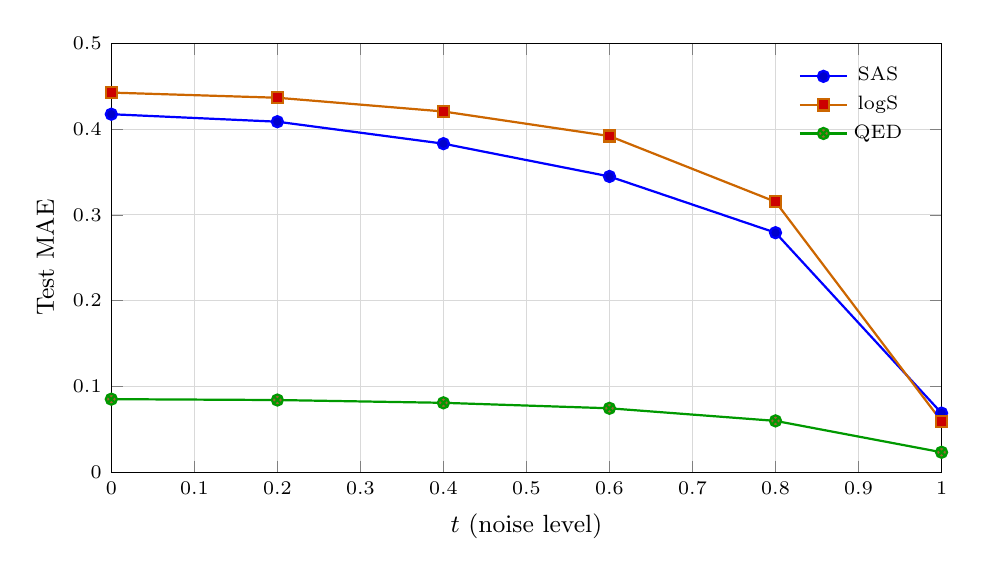
\begin{tikzpicture}
\begin{axis}[
  width=\columnwidth,
  height=0.58\columnwidth,
  xlabel={$t$ (noise level)},
  ylabel={Test MAE},
  xmin=0, xmax=1,
  ymin=0, ymax=0.5,
  grid=both,
  grid style={line width=0.3pt, draw=gray!30},
  tick label style={font=\scriptsize},
  label style={font=\small},
  legend style={font=\scriptsize, draw=none, fill=none},
  legend pos=north east,
]
\addplot+[thick, blue] coordinates {
  (0.0, 0.4171967224)
  (0.2, 0.4084696747)
  (0.4, 0.3828861816)
  (0.6, 0.3446883911)
  (0.8, 0.2791697571)
  (1.0, 0.0690200127)
};
\addlegendentry{SAS}

\addplot+[thick, orange!80!black] coordinates {
  (0.0, 0.4423901184)
  (0.2, 0.4363820099)
  (0.4, 0.4203746033)
  (0.6, 0.3917442139)
  (0.8, 0.3152096558)
  (1.0, 0.0594828186)
};
\addlegendentry{logS}

\addplot+[thick, green!60!black] coordinates {
  (0.0, 0.0852654148)
  (0.2, 0.0842592201)
  (0.4, 0.0810060917)
  (0.6, 0.0746299919)
  (0.8, 0.0599623322)
  (1.0, 0.0234130266)
};
\addlegendentry{QED}
\end{axis}
\end{tikzpicture}
\caption{\footnotesize Test MAE of time/noise-conditioned property regressors versus noise level $t$
(0 = fully noised, 1 = clean/denoised). Each point averages 10k test molecules. Errors are large for
noisy inputs and only reasonable at $t=1$.}
\label{fig:regressor-noise}
\end{figure}
